\newpage
\section{Analisi dei Risultati}
\label{section:analisirisultati}

%1 test: Questa proprietà lo penalizza nelle simulazioni che sono 





In quest'ultima analisi, invece, verrà mostrata un'interazione tra 2 diversi gruppi di utenti (Nodi).
Il primo gruppo è formato da persone con un'alta probabilità di condividere la notizia 
mentre nel secondo, al contrario, da persone con una bassa probabilità.
Questo studio punta ad analizzare quante visualizzazioni vengono fatte per una singola informazione condivisa.
Verrà anche condotto uno studio in cui il totale degli utenti si divide in due gruppi costituiti da, ad esempio, 
pochi utenti con alte probabilità di condividere l'informazione e, viceversa, 
molti utenti con basse probabilità di condivisione.
La possibilità di condivisione è data nuovamente dal confronto tra 
la ``forza della notizia'' e la ``forza di astensione''. 
In questo caso, però, l'astensione viene calcolata tramite una funzione di distribuzione di probabilità non lineare,
quella scelta è la funzione Weibull.
La funzione ``random-weibull'' fa variare, per mezzo dei due parametri $\alpha$ e $\beta$, la pendenza della distribuzione
e, di conseguenza, anche la sua densità.




Per ottenere una curva di distribuzione più o meno inclinata, in seguito ai tentativi attuati, 
è stato ritenuto opportuno mantenere il valore di $\beta$ costante a 1.0 e variare, invece, quello di $\alpha$.



%----

\begin{figure}[!ht]
\centerline {
  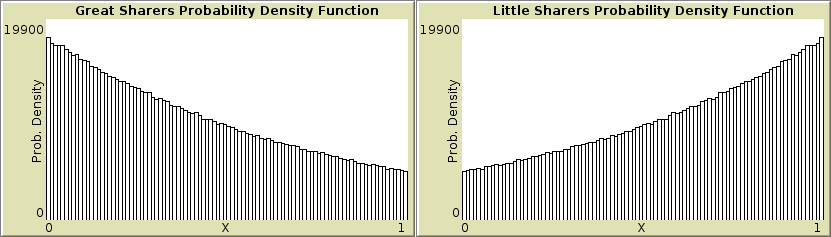
\includegraphics[width=1.1\textwidth]{img/weibull-alpha-0.75.png}
}
\caption{I due istogrammi mostrano la rappresentazione di un vettore $X$ di 1 milione di cifre 
calcolato mediante la funzione di densità di probabilità Weibull, con $\alpha = 0.75$.
Il grafico di sinistra rappresenta la distribuzione originale, 
mentre quello di destra la sua speculare calcolata grazie: $\forall x \in X, \quad 1 - x$.}
\label{img:weibull_alpha_0_75}
\end{figure}

Nella figura~\ref{img:weibull_alpha_0_75} il dislivello non è troppo alto e questo permette 
comunque al gruppo 2 un buon grado di condivisione della notizia.

Questa analisi è stata sviluppata mediante tre cicli annidati che hanno considerato tutte le 
possibilità che verranno di seguito esposte.\\
Il primo ciclo più esterno itera su alcuni valori di forza della notizia, 
ovvero i seguenti: $0.50 \quad 0.60 \quad 0.70 \quad 0.75 \quad 0.80 \quad 0.90$.\\
Il secondo ciclo, quello centrale, modifica il numero di individui per ogni gruppo. 
Ad ogni passo viene incrementato il numero di persone con un'alta possibilità di condivisione 
passando dal 10\% al 90\%. Operazione inversa viene eseguita per le persone con bassa possibilità di 
condivisione passando dal 90\% al 10\% della popolazione totale.
Il terzo ciclo, più interno, invece itera sul parametro $\alpha$ modificando quindi la pendenza della 
curva per gli individui con alta probabilità di condivisione.

Il test viene composto da i parametri dinamici appena citati e dai seguenti parametri statici:
\begin{itemize}
\item La dimensione della popolazione non cambia mai e resta sempre di 500 Nodi;
\item Il parametro $\alpha$ del gruppo con bassa probabilità di condivisione rimane $0.75$, 
ottenendo una densità di probabilità come in figura \ref{img:weibull_alpha_0_75};
\item La topologia del grafo è la stessa per ogni esecuzione del test;
\end{itemize}

Il risultato di ogni test inoltre viene mediato sull'esito di 500 test.


%----


La figura \ref{img:last_test_str_0_5} mostra il risultato atteso, 
ovvero la crescita del numero di visualizzazioni sia al variare di $\alpha$ che all'aumentare 
dei nodi con alta probabilità di condivisione.

Si vuole inoltre porre l'attenzione su come con un valore di $\alpha$ 
molto basso ($0.2$) ed un numero di nodi con alta probabilità di condivisione pari a 150 corrisponda 
a ~ 300 visualizzazioni totali, quasi le stesse ottenute da un valore di $\alpha$ = 1.0 e 325 nodi con 
alta probabilità di condivisione.




\begin{figure}[!ht]
\centerline {
  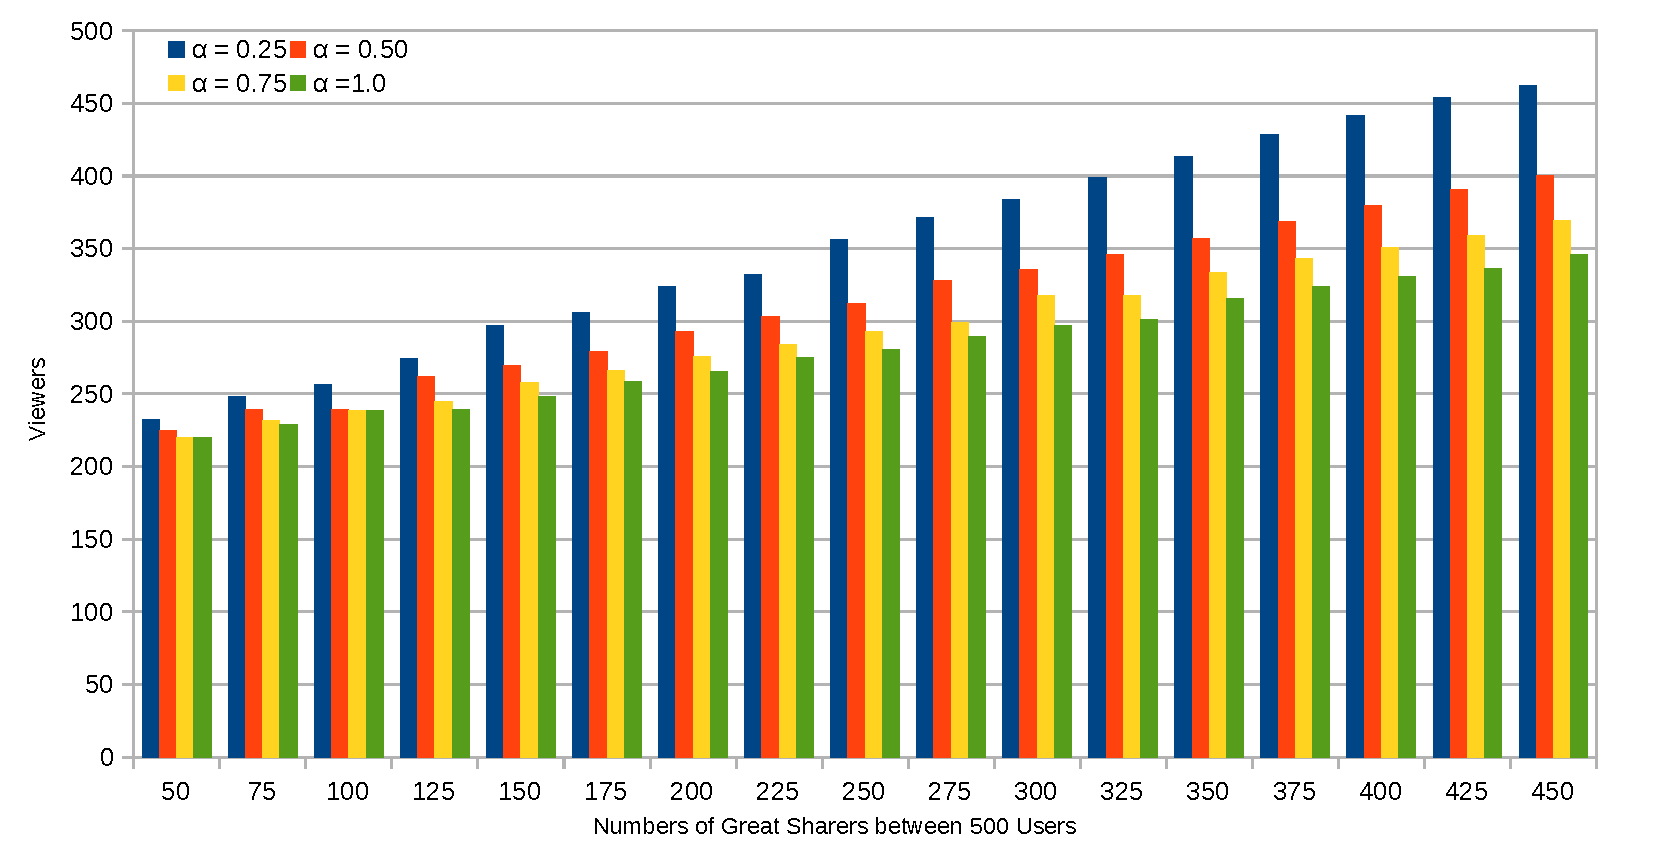
\includegraphics[width=1.1\textwidth]{charts/last-test-str_0.5.pdf}
}
\caption{Grafico del risultato dell'ultimo test con forza della notizia pari a $0.50$, 
500 nodi totali e $\alpha$ del gruppo con bassa probabilità di condivisione = $0.75$}
\label{img:last_test_str_0_5}
\end{figure}











